\chapter{Aplicaci\'on de Prueba}
Una vez finalizada la tarea de implementaci\'on del motor combinatorio, se continua con la elaboraci\'on de una aplicaci\'on sencilla cuya \'unica
finalidad es la comprobaci\'on de que el motor funcione de la manera esperada.

Esta aplicaci\'on, de nombre \textbf{Clothes Changer}, no requiere distribuci\'on de su trabajo debido a la simpleza en sus c\'alculos, pero a\'un as\'i es
de gran utilidad para poder probar algunas pol\'iticas de combinaci\'on como as\'i tambi\'en observar la nueva capa acoplada a \fud.

\section{Descripci\'on Del Problema}
A partir de un conjunto de prendas de vestir, se desea conocer todas las posibles maneras en que una persona puede vestirlas, es decir, armar todas
las combinaciones del conjunto de ropas. Adem\'as, se quiere hacer un ``ranking'' con las mejores 5 vestimentas.

Cada prenda pertenece a una de las siguientes categor\'ias (notar que una vestimenta es factible siempre y cuando est\'e consituida por una prenda de
cada una de estas categor\'ias).
\begin{itemize}
  \item Pantalones.
  \item Remeras.
  \item Medias.
  \item Calzados.
\end{itemize}

\section{Soluci\'on}
Debido a que la aplicaci\'on fue pensada como un caso de estudio simple para el motor combinatorio, la misma ha sido implementada respetando la interface
que \combeng \ propone. La soluci\'on planteada puede ser descompuesta en dos partes:
\begin{itemize}
  \item Generar todas las posibles vestimentas.
  \item Calcular un puntaje o \textit{score} para cada vestimenta, representando qu\'e tan buena es la combinaci\'on de prendas.
\end{itemize}

\subsection{Generaci\'on De Vestimentas}
Para generar todas las posibles vestimentas se utiliza una pol\'itica de combinaci\'on paralela (ver \ref{composedCombPolicyParallel}), donde cada pol\'itica
simple que la compone es del tipo \emph{ListCombinationPolicy}, cada una actuando sobre una \'unica categor\'ia de ropa.
\begin{center}
  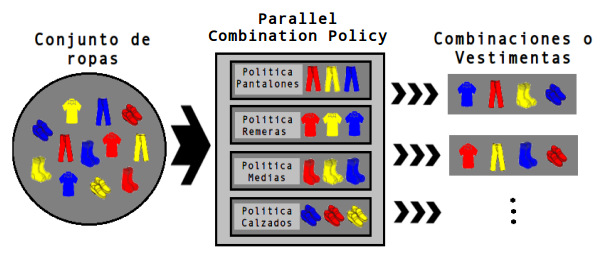
\includegraphics[width=\linewidth]{images/sequencial_ropa.png} 
\end{center}
\newpage
\subsection{C\'alculo Del Score Para Una Vestimenta}
Las tablas que se muestran a continuaci\'on determinan qu\'e tan bien ``combinan'' dos prendas (un pantal\'on con una remera, o un pantal\'on con un
par de medias, etc.). El valor o puntaje de una vestimenta se obtiene realizando la suma entre las diferentes tablas, a partir de las prendas de
vestir que la componen (las tablas fueron inicializadas con valores aleatorios). \\

\textbf{\emph{Tabla Remera-Pantal\'on}}\\

\begin{tabular}{|c|c|c|c|c|}
  \hline Ropa y Color        & Rem. Blanca & Rem. Amarilla      & Rem. Roja  & Rem. Azul \\ 
  \hline Pant. Blanco   & 5           & 2                & 4            &  7          \\
  \hline Pant. Amarillo & 4           & 5                & 6            &  4          \\ 
  \hline Pant. Rojo     & 4           & 4                & 2            &  7          \\ 
  \hline Pant. Azul     & 3           & 5                & 4            &  9          \\  
  \hline 
\end{tabular}

\vspace*{.9cm}
\textbf{\emph{Tabla Pantal\'on-Medias}}\\

\begin{tabular}{|c|c|c|c|c|}
  \hline Ropa y Color      & Pant. Blanco 	   & Pant. Amarillo	     & Pant. Rojo      & Pant. Azul \\ 
  \hline Med. Blancas      & 3           	   & 6               & 9               &  7          \\
  \hline Med. Amarillas    & 5               & 1               & 2               &  9          \\ 
  \hline Med. Rojas        & 4               & 5               & 3               &  1          \\ 
  \hline Med. Azules       & 2               & 4               & 8               &  4          \\  
  \hline 
\end{tabular}

\vspace*{.9cm}
\textbf{\emph{Tabla Medias-Calzados}}\\

\begin{tabular}{|c|c|c|c|c|}
  \hline Ropa y Color      & Med. Blancas & Med. Amarillas      & Med. Rojas & Med. Azules \\ 
  \hline Cal. Blanco    & 6           & 2                & 7            &  1          \\
  \hline Cal. Amarillo  & 3           & 4                & 3           &  2          \\ 
  \hline Cal. Rojo      & 8           & 7                & 6            &  8          \\ 
  \hline Cal. Azul      & 1           & 9                & 2            &  3          \\  
  \hline 
\end{tabular}

\vspace*{.9cm}
A modo de ejemplo, supongamos que una vestimenta generada por el motor combinatorio consta de las siguientes prendas:
\begin{itemize}
  \item \emph{Remera Azul}
  \item \emph{Pantal\'on Blanco}
  \item \emph{Medias Rojas}
  \item \emph{Calzado Blanco}
\end{itemize}
Para calcular el score de esta vestimenta, indexamos las tablas de acuerdo a las ropas que la componen y sumamos los valores. En este caso:

\begin{itemize}
  \item \emph{Remera Azul} y \emph{Pantal\'on Blanco}  = \textbf{7}
  \item \emph{Pantal\'on Blanco} y \emph{Medias Rojas} = \textbf{4}
  \item \emph{Medias Rojas} y  \emph{Calzado Rojo}    = \textbf{6}
\end{itemize}
Dando un valor para la vestimenta de \emph{ \textbf{17}}.
